\addbibresource{reference.bib}

\chapter{Úvod do hybridních částicových pixelových detektorů}\label{chap:detectors}
Ionizující záření je lidskými smysli nedetekovatelné, avšak jeho studium nám umožňuje pochopit podstatu hmoty, její vlastnosti a interakce. To lidstvu umožnilo mnohé aplikace, jako je například protonová terapie \cite{tpx_app_radiotherapy}, defektoskopie nebo zkoumání pravosti uměleckých děl. První pokusy o detekci ionizujícího záření sahají do počátku 20. století, kde se pomocí mlžné komory prvně podařilo zachytit trajektorii nabitých částic. Rozvoj polovodičové technologie dal vzniku novým detekčním technologiím až po v současné době nejpokrokovějším - pixelovým detektorům.

Existuje celá řada částicových pixelových detektorů, ale v této kapitole budou popsány jen hybridní pixelové detektory, pro které je typické, že se skládají ze dvou nezávisle vyrobených částí - senzoru a vyčítacího čipu. To oproti monolitickým detektorů, kde vyčítací elektronika je součástí senzoru přináší řadu výhod, jako například snížení výrobních nákladů nebo možnost kombinace vyčítacího čipu se senzory různých materiálů (\textit{Si}, \textit{GaAs}, \textit{CaTe} apod.) a tlouštěk (vetšinou $300\mu m$, nebo $500\mu m$).

Na tomto místě je třeba zmínit, že existuje více druhů těchto detektorů (\textit{AGH Fermilab, Pilatus, Philips Chromaix} apod.)\cite{detectors_review}, v této práci budou použity pouze detektory z rodiny detektorů Medipix.

%********************************************************************************
% Hardwarová architektura
%********************************************************************************
\section{Hardwarová architektura}
\begin{figure}[th]
	\begin{center}
		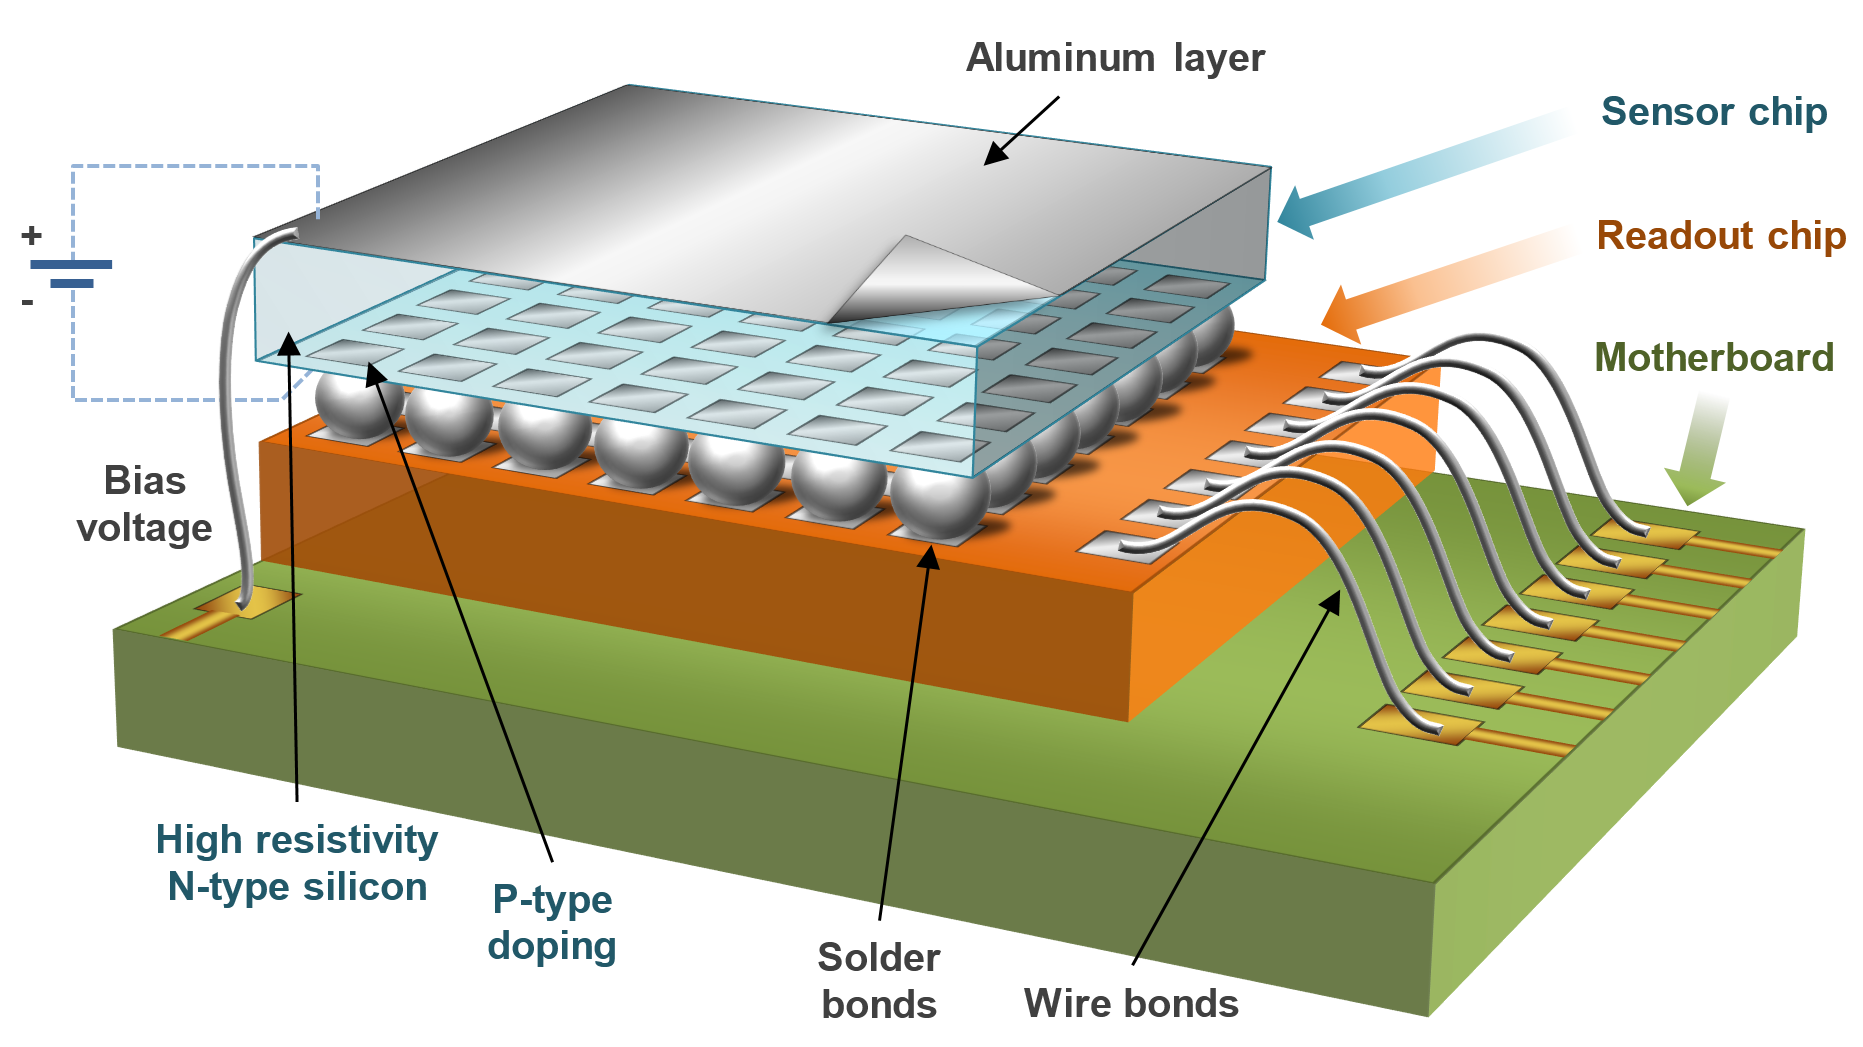
\includegraphics[width=12cm]{figures/det_chip.png}
		\caption{Struktura hybridního polovodičového pixelového detektoru Timepix3, skládající se z vyčítacího čipu a polovodičového senzoru \cite{PlatkevicDisertace}.}
		\label{fig:det:chip}
	\end{center}
\end{figure}
Většina hybridních částicových pixelových detektorů rodiny Medipix obsahuje matici $256\times256$ pixelů. Každý z nich má stanu o délce $55~\mu m$, takže senzor čítající $65536$ má plochu $1.4 \times 1.4 cm^2$. 

Na obrázku \ref{fig:det:chip} je znázorněna struktura detektoru Timepix3. Vrchní část detektoru tvoří polovodičový senzor, který je nejčastěji vyroben z křemíku, ale výjimkou není také \textit{GaAs} nebo \textit{CaTe}. Jednotlivé pixely senzoru jsou spojeny s integrovaným \texttt{ASIC}\footnote{z angl. Application Specific Integrated Circuit} vyčítacím čipem pomocí technologie zvané \textit{Bump-Bounding}. Vyčítací čip je pak propojen se základní deskou pomocí \textit{wire-bound}, z které je ještě přivedeno měřící napětí na senzor detektoru (tzv. \textit{bias}).


%********************************************************************************
% Princip detekce
%********************************************************************************
\section{Princip detekce}\label{chap:detectors:princip}
\begin{figure}[th]
	\begin{center}
		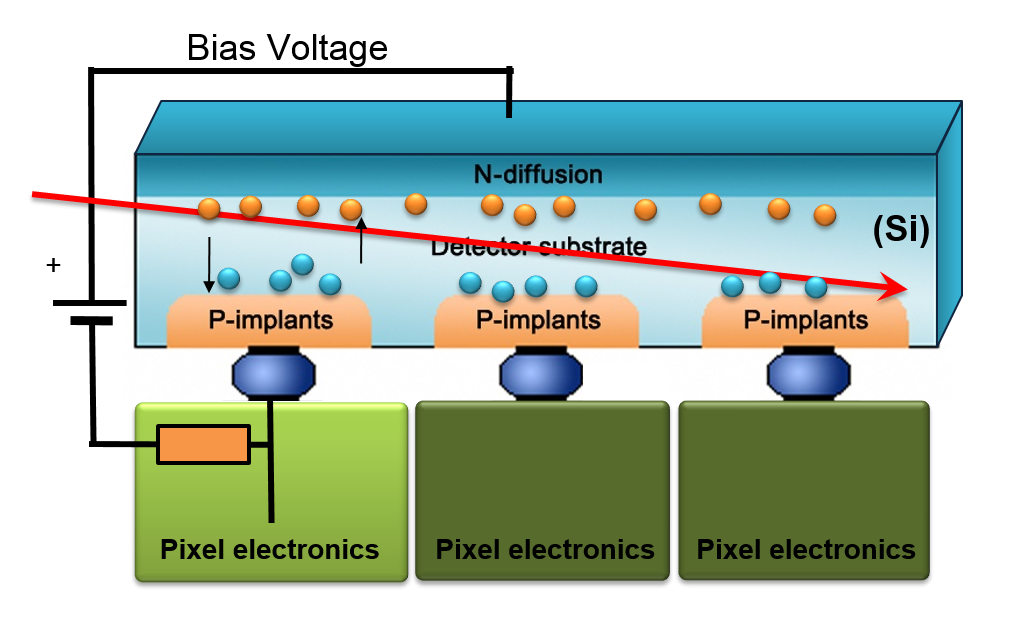
\includegraphics[width=10cm]{figures/det_recombination.png}
		\caption{Princip detekce ionizujícího záření detektorem Timepix3 \cite{PlatkevicDisertace}.}
		\label{fig:det:recombination}
	\end{center}
\end{figure}

Princip detekce ionizujícího záření pixelovými detektory je založen na známém jevu detekce ionizujícího záření v polovodiči. 

Jako náhradní schéma jednoho pixelu si lze představit diodu zapojenou v závěrném směru, kterou bez přítomnosti ionizujícího záření protéká minimální proud. Vnikne-li do senzoru ionizující částice a dojde k její interakci se senzorem, resp. část její energie je deponována do polovodičového objemu senzoru, dojde v senzoru ke vzniku elektron-děrových páru a díky lavinovému efektu i k následnému otevření PN přechodu (viz na obr. \ref{fig:det:recombination}, kde červená šipka znázorňuje interagující částici, elektrony jsou znázorněny žlutě, modře díry).

Vzniklý proudový impulz je měřícím odporem převeden na napětí, které je komparátorem porovnáno s prahovým napětím (tzv. \textit{threshold}). Výsledek této komparace je dále CMOS\footnote{Z angl. \textit{Complementary Metal–Oxide–Semiconductor}, výrobní technologie logických integrovaných obvodů.} obvodem zpracován, dle použitého měřícího módu, jak bude ukázáno v kapitole \ref{chap:detectors:operation_modes}.

Na rozdíl od CCD\footnote{Z angl. \textit{Charge-coupled device}.} technologie, CMOS readout \textit{Timepix}/\textit{Medipix} detektorů negeneruje temný proud\footnote{Termín charakterizující vyčítací šum u CCD snímačů. Obvykle je udáván v elektronech za sekundu při konstantní teplotě a ve tmě.}, díky odstínění signálu od šumu pomocí komparačního napětí. To znamená, že doba jedné akvizice je teoreticky neomezena, protože detektor je schopný detekovat jen ty částice, jejíchž deponovaná energie (resp. amplituda vzniklého napěťového pulzu) je větší, než \textit{threshold}.

%********************************************************************************
% Operační módy detektoru
%********************************************************************************
\section{Operační módy detektoru}\label{chap:detectors:operation_modes}
\begin{figure}[th]
	\begin{center}
		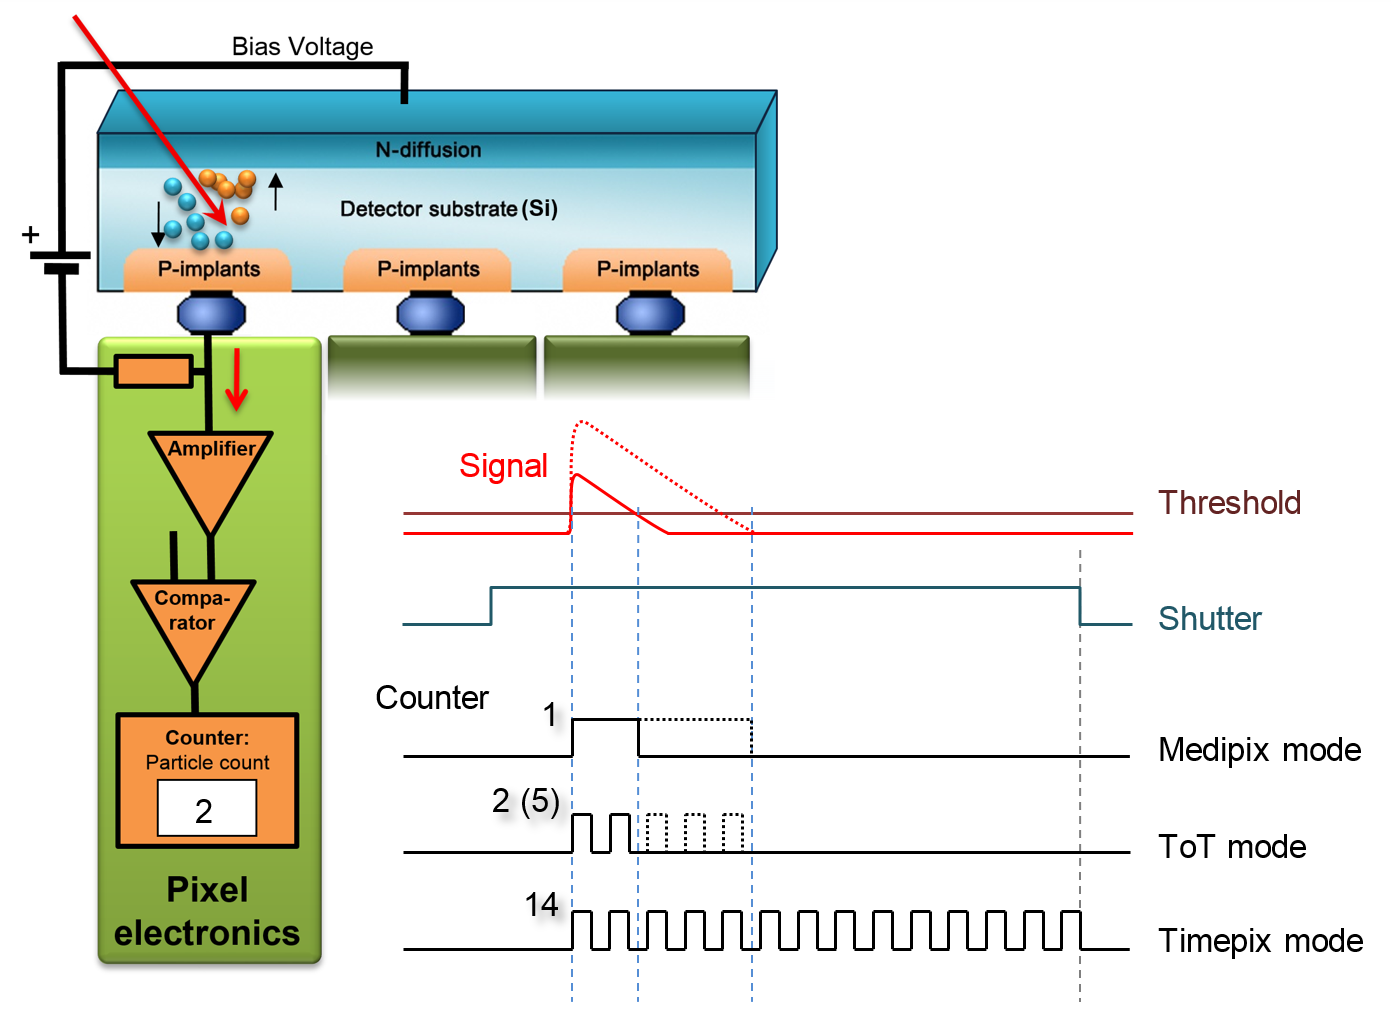
\includegraphics[width=14cm]{figures/det_pix.png}
		\caption{Zpracování signálu pixelem detektoru dle nastaveného módu (\textit{Medipix}, \textit{ToT} a \textit{ToA}) \cite{PlatkevicDisertace}.}
		\label{fig:det:modes}
	\end{center}
\end{figure}


V této podkapitole bude vysvětlena většina operačních módu, ve kterých detektory rodiny \textit{Medipix} jsou schopny pracovat. 

Jak už bylo popsáno v předchozí kapitole, interagovaná částice vyvolá napěťový impulz, jehož tvar koreluje s deponovanou energií. Pro účely analýzy se ale používá pouze binární informace o překročení prahového napětí v čase. Výsledek této analýzy je po jejím dokončení uložen ve 14-bitovém registru pixelu.

Na obr. \ref{chap:detectors:operation_modes} je znázorněn příklad zpracování analýzy signálu následujícími módy:
\begin{description}
    \item[Medipix mód (Counting mód)] V tomto módu je čítač inkrementován v každém cyklu měřící frekvence, pokud měřící napětí překročilo prahové napětí pixelu. Na konci akvizice pak hodnota čítače odpovídá počtu zaznamenaných částic.
    \item[Time-Over-Threshold (ToT)] Pracuje-li pixel v tomto módu, pak jeho čítač je inkrementován v každém cyklu měřící frekvence, pokud měřící napětí je vyšší, než prahové napětí pixelu. Hodnota uložená v čítači odpovídá deponované energii interagovaných částic. Mezi energií a \texttt{ToT} je nelineární závislost a její zkoumání je předmětem energetické kalibrace detektoru, jak bude ukázáno v kapitole \ref{chap:detectors:calibration:energy}. Tento mód má široké spektrum aplikací, například \cite{tot_app_counting} nebo \cite{tpx_app_radiotherapy}.
    \item[Time-of-Arrival (ToA)] Tímto módem disponují pouze detektory \textit{Timepix} a \textit{Timepix3}, avšak nesdílí stejný princip. Zatímco \textit{Timepix} detektor začne inkrementovat čítač v každém cyklu měřící frekvence po první náběžné hraně z komparátoru, \textit{Timepix3} na náběžnou hranu uloží do 14-bitového registru aktuální časové razítko z hodin detektoru. V obou případech \texttt{ToA} udává čas první interakce částice v dané akvizici.
\end{description}

%********************************************************************************
% Vyčítání naměřených dat
%********************************************************************************
\section{Vyčítání naměřených dat}\label{chap:detectors:readout}
Jednotlivé detektory rodiny \textit{Medipix} mají různou hardwarovou podporu pro vyčítání naměřených dat. Detektory vždy podporují alespoň jeden z těchto módů:
\begin{description}
	\item[Frame-Based] Pracuje-li detektor v tomto módu, pak jsou všechny registry čítačů pixelů vyčítány najednou, po dokončení aktuálního snímku. Vždy je třeba vyčíst všechny pixely bez ohledu na naměřenou hodnotu.
	\item[Data-Driven] Tento mód, také označovaný jako \textit{Event-Driven}, byl prvně použit v detektoru \textit{Timepix3}. Pracuje-li detektor v tomto módu, pak v průběhu akvizice dat (resp. když \textit{shutter} signál je nastaven na úroveň \texttt{HIGH}) každý pixel po zpracování události notifikuje readout interface o tom, že nová data jsou připravena k vyčtení a readout interface je pak bez prodlení vyčte a dále zpracuje.
\end{description}

Na obrázku \ref{fig:det:frame_vs_event_driven} je vidět hlavní motivace pro zavedení podpory \textit{Data-Driven} módu u detektoru \textit{Timepix3}. Ukázalo se, že \textit{Data-Driven} mód je efektivnější při takových měření, kde okupance snímků je menší než zhruba $50\%$. Po překročení této meze je efektivnější použití \textit{Frame-Based} módů, protože není třeba přenášet souřadnice zasažených pixelů. Podle \cite{timepix3} vyčítací čas může být definován následovně:
\begin{equation}\label{eq:det:readout_time}
	T_{readout} = N_{pixels}*bits_{pixel}/BW
\end{equation}
kde:
\begin{changemargin}{1.5cm}{1cm} 
	\begin{itemize}
		\item[$N_{pixels}$] je počet pixelů které je potřeba vyčíst (pro \textit{Frame-Based} mód jsou to všechny pixely detektoru ($256\times256$) a pro \textit{Data-Driven} je to počet zasažených pixelů),
		\item[$bits_{pixel}$] je počet bitů na pixel ($28 b$ v \textit{Frame-Based} módu a $28b + 16b$ v \textit{Data-Driven} módu kvůli nutnosti přenášení adresy pixelu) a
		\item[$BW$] je počet bytů za vteřinu, které je možné vyčíst z detektoru (\textit{bandwidth}). 
	\end{itemize}
\end{changemargin}

\begin{figure}[th]
	\begin{center}
		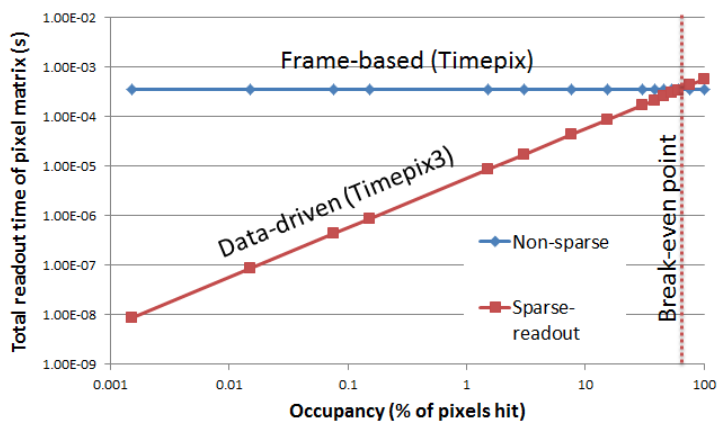
\includegraphics[width=14cm]{figures/det_frame_vs_event_driven.png}
		\caption{Doba vyčítání detektoru za použití \textit{Frame-based} (non-sparse) a \textit{Data-driven} (sparse) módu \cite{timepix3}.}
		\label{fig:det:frame_vs_event_driven}
	\end{center}
\end{figure}

%********************************************************************************
% Kalibrace
%********************************************************************************
\section{Kalibrace}\label{chap:detectors:calibration}
Každý detektor má své specifické vlastnosti, které jsou dány nejenom výrobním procesem, ale i závislostí na opotřebení a únavě materiálu v čase, okolní teplotě nebo na nastavených měřících parametrech (například \textit{bias}). Hlavní motivací pro kalibraci detektorů je minimalizace systematické chyby měření. Z pohledu aplikace získaných kalibračních dat je možné kalibrační metody rozdělit do dvou kategorií:
\begin{enumerate}[label=(\roman*)]
	\item Použití v průběhu akvizice dat - jedná se o data, která jsou použita pro nastavení akvizice dat v detektoru a mají přímý vliv na naměřená data, která danou metodou není možné dodatečně kalibrovat. Do této kategorie spadá například \textit{treshold equalizace} (viz \ref{chap:detectors:calibration:equalization}).
	\item Transformace naměřených dat - v tomto případě jsou kalibrační data aplikovaná dodatečně na naměřená data. Tento přístup má výhodu v možnosti dodatečné kalibrace již naměřených dat. Do této kategorie spadá například \textit{Energetická kalibrace} (viz \ref{chap:detectors:calibration:energy}) nebo \textit{Time-Walk korekce} (viz \ref{chap:detectors:calibration:timeWalk}).
\end{enumerate}

\subsection{Treshold equalizace}\label{chap:detectors:calibration:equalization}
V podkapitole \ref{chap:detectors:princip} a \ref{chap:detectors:operation_modes} již bylo vysvětleno použití prahového napětí (\textit{treshold}) v průběhu akvizice dat detektorem. Každý pixel detektoru má ale rozdílné fyzikální vlastnosti dané výrobním procesem, s čímž souvisí i citlivost (resp. oddělení užitečného signálu od šumu) jednotlivých pixelů. Kromě globální hodnoty tresholdu je možné pro každý pixel upravit citlivost pomocí lokální $4b$ hodnoty tresholdu (viz obr. \ref{fig:det:medipix_overview:timepix3_schema}).

Vlastní proces equalizace probíhá tak, že se udělá treshold scan přes všechny hodnoty, přičemž je třeba minimalizovat interakce detektoru z částicemi. V běžné praxi stačí detektor dostatečně odstínit. Výstupem tohoto procesu je pak globální treshold a jeho 4-bitové korekce pro jednotlivé pixely.

Jako vedlejší produkt tohoto procesu je rovněž maskovací matice detektoru, které obsahuje šumějící, nebo jinak poškozené pixely. To jsou například takové pixely, které bez přítomnosti interagujících částic hlásí překročení tresholdu.

\subsection{Energetická kalibrace}\label{chap:detectors:calibration:energy}
\begin{figure}[th]
	\begin{center}
		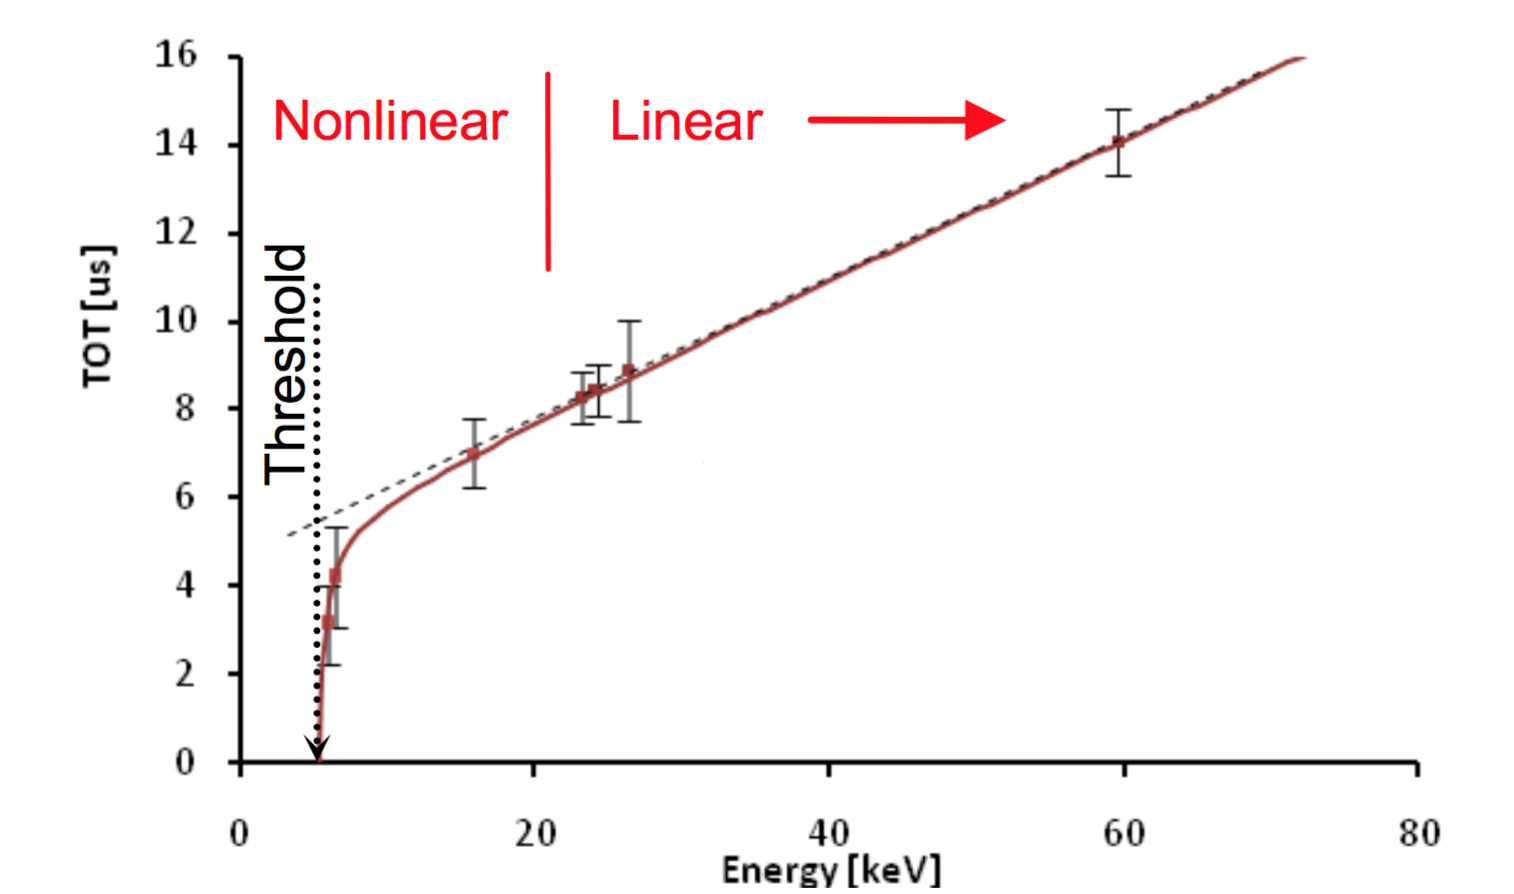
\includegraphics[width=13cm]{figures/calib_function.png}
		\caption{Kalibrační funkce, udávající závislost mezi energií v \texttt{keV} a \texttt{ToT} \cite{Jakubek2011S262}, vzniklá proložením získaných kalibračních bodů funkcí \ref{eq:det:energyCalib} a sestávající se ze dvou částí - (i) nelineární částí pro oblast nižších energií (hyperbola) a (ii) lineární částí pro vyšší energie (přijímka).}
		\label{fig:det:calib:calib_function}
	\end{center}
\end{figure}

V předchozí části práce byl již představen \textit{Time-Over-Treshold} mód (viz \ref{chap:detectors:operation_modes}), ve kterém je detektor schopný měřit deponovanou energii interagovaných v částic, která je udávána v \texttt{ToT}. Jak již bylo ukázáno, vztah mezi energií v \textit{keV} a \texttt{ToT} je nelineární závislost a závisí na fyzikální vlastnostech daného pixelu, což je předmětem energetické kalibrace, která bude v této podkapitole popsána.

Tato metoda \cite{Jakubek2011S262} spočívá v provedení několika sad měření se zdroji ionizujícího záření, jejichž energie jsou předem známy, a v jejich analytickém zpracování a vytvoření kalibrační funkce \ref{eq:det:energyCalib} pro každý pixel detektoru. V předchozí práci \cite{BegeraBcThesis2016} byly tyto metody podrobně popsány a byl vytvořen software, který uživateli umožňuje vytvoření energetické kalibrace detektoru z naměřených dat.

\begin{equation}\label{eq:det:energyCalib}
	f_{calib}(x) = ax + b - \frac{c}{x-t}
\end{equation}

Pro měření kalibračních dat se jako efektivní řešení v praxi ukázalo použití rentgenové fluorescence\footnote{Děj, ke kterému dochází při ozařování materiálu (nejčastěji \textit{Cu}, \textit{Fe}, \text{In} apod.) rentgenovým zářením, při kterém jsou z něj vyráženy excitované elektrony. Při vyražení elektronu na nižší energetické úrovni, elektron z vyšší energetické úrovně obsadí jeho místo a přebytečnou energii emituje formou vyzářeného fotonu - fluorescenčního záření, jehož charakteristické monoenergetické spektrum je pro většinu prvků dobře známé.} \cite{Jakubek-radiography_and_charge_sharing}. Pro zajištění dobré kvality kalibrace je třeba naměřit takový počet událostí, aby spektra ve snímcích byla dobře rozeznatelná. Z naměřených dat jsou vyfiltrovány pouze tzv. \textit{Single-hit} události\footnote{Události, ve kterých částice interagovala pouze s jedním pixelem detektoru}, aby se minimalizovaly negativní vlastnosti \textit{Charge-sharing} efektu (díky společné elektrodě senzoru jsou díky interagující částici vzniklé elektrony zpracovány více pixely najednou a část deponované energie nemusí být ASIC čipem zpracována, protože vzniklý signál může být nižší než treshold daného pixelu).

\begin{figure}[th]
	\begin{center}
		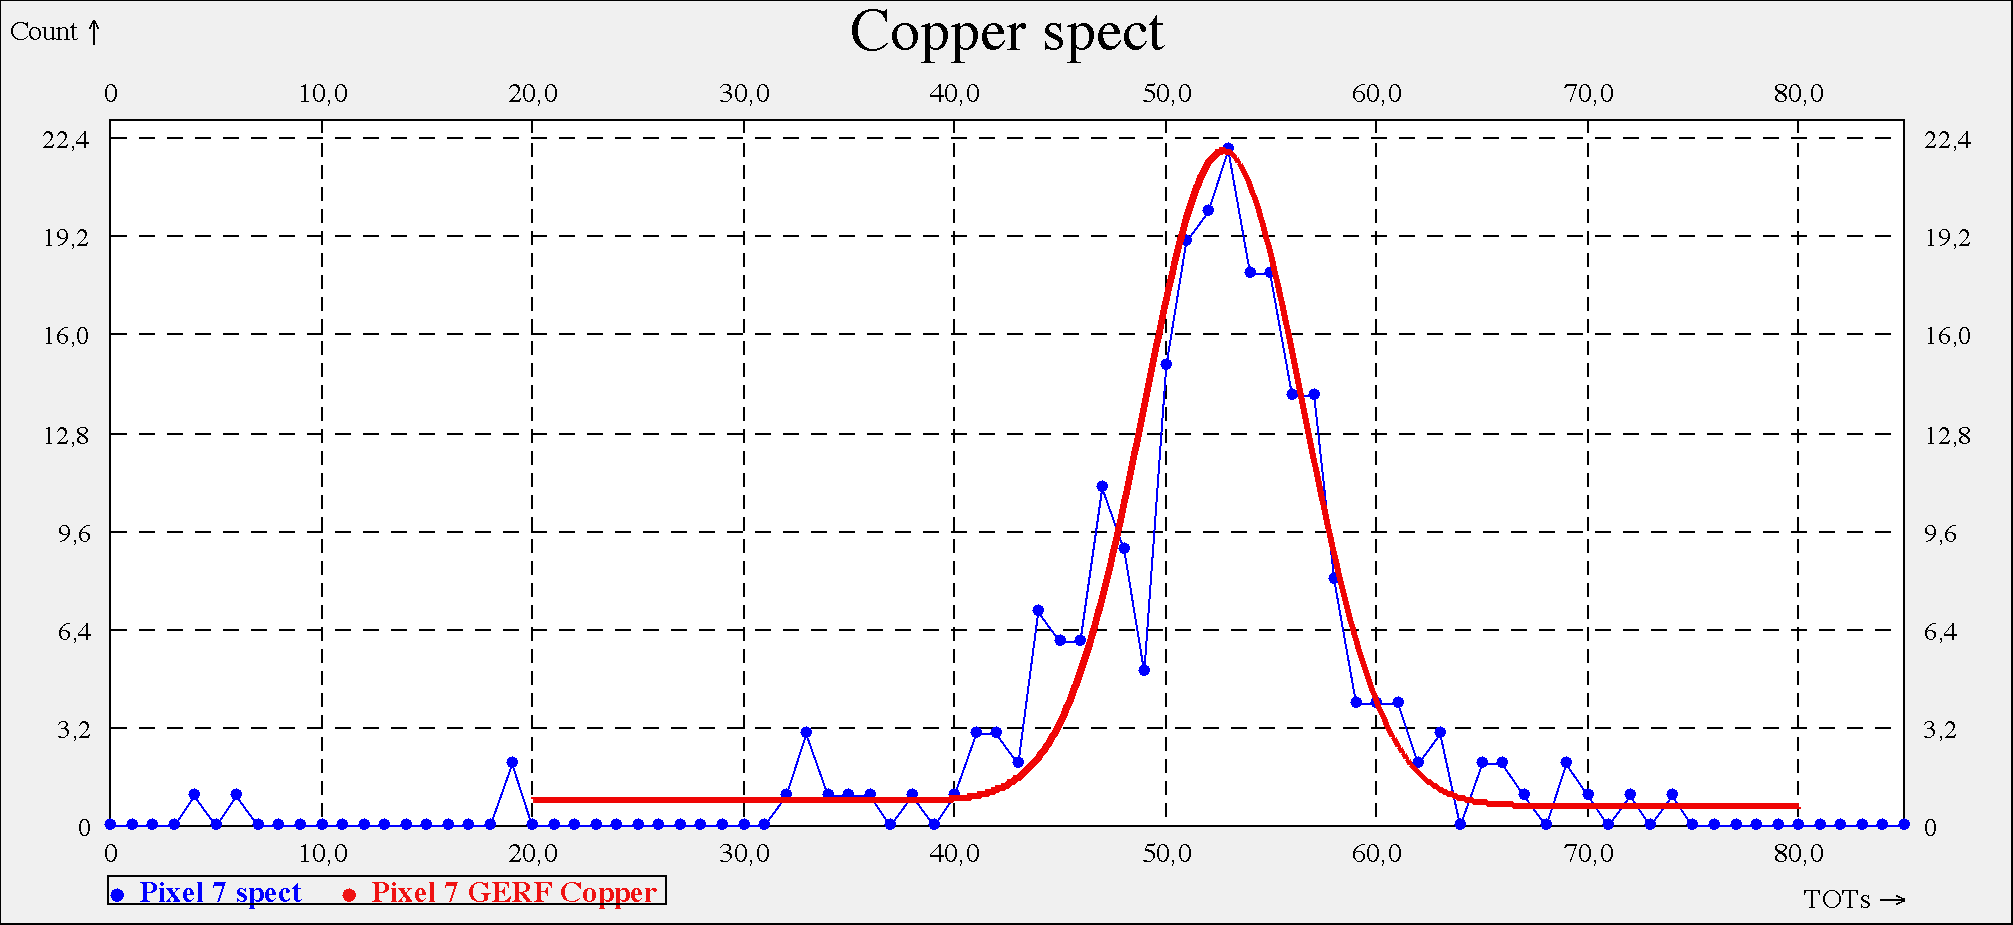
\includegraphics[width=15cm]{figures/calib_gerf.png}
		\caption{Příklad energetického spektra jednoho pixelu Timepix detektoru s proloženou funkcí \ref{eq:det:gerf} \cite{BegeraBcThesis2016}.}
		\label{fig:det:calib:gerf}
	\end{center}
\end{figure}

Z jednotlivých měření jsou pro každý pixel detektoru vytvořena spektra \texttt{ToT} hodnot. Na obrázku \ref{fig:det:calib:gerf} je znázorněn příklad takového spektra, získaného z fluorescence mědi. Požadovaný kalibrační bod se získá střední hodnoty \texttt{ToT} a tabulkové hodnoty energie fluorescenčního záření mědi. Střední hodnota je získána proložením spektra funkcí \ref{eq:det:gerf} - jedná se o součet Gaussovy funkce a Gaussovy chybové funkce (kvůli levé nesymetrii vzniklé \textit{Charge-sharing} efektem)
\begin{equation}\label{eq:det:gerf}
	f_{GERF}(x) = \underbrace{Ae^{ -\frac{(x-\mu)^2}{2\sigma^2} }}_{\text{Gaussova funkce}} +
	\underbrace{ \frac{avg_{right} - avg_{left}}{\sigma\sqrt{2\pi}} \int_{-\infty}^t e^{ -\frac{(t-\mu)^2}{2\sigma^2} } + avg_{left}}_{\text{Gaussova chybová funkce}},
\end{equation}
kde:
\begin{changemargin}{1.5cm}{1cm} 
	\begin{itemize}
		\item [$A$] je amplituda,
		\item [$\mu$] je stření hodnota hledané energie,
		\item [$\sigma$] je rozptyl střední hodnoty energie $\mu$, který je možné vypočítat ze vzorce 
			\ref{eq:det:gerf_sigma}, kde \texttt{FWHM}\footnote{z angl. Full Width at Half Maximum} udává šířku gausiánu v~polovině jeho výšky a
		\item [$avg_{right}$, $avg_{left}$] je průměrná hodnota spektra na pravém (resp. levém) úpatí gausiánu.
	\end{itemize}
\end{changemargin}

\begin{equation}\label{eq:det:gerf_sigma}
	\sigma = \frac{2\sqrt{2ln_2}}{FWHM}
\end{equation}

\subsection{Time-Walk korekce}\label{chap:detectors:calibration:timeWalk}

\textit{Time-Walk} efekt je nežádoucí jev, který vzniká při interakci ionizujícího záření o různé energii. Velikost deponované energie má vliv na amplitudu a sklon napěťového pulzu na zesilovači pixelu. Při interakci ionizující částice s více pixely je pak díky tomuto jevu interagovanými pixely zaznamenána jiná hodnota \textit{Time-of-Arrival} (ToA), i přes to že událost byla způsobena stejnou částicí a ToA by měl být stejný. Viz obrázek \ref{fig:det:calib:timeWalk}, kde jsou pro interakci stejné částice čtyřmi sousedními pixely zaznamenány různé hodnoty ToA. 

\begin{figure}
	\begin{center}
		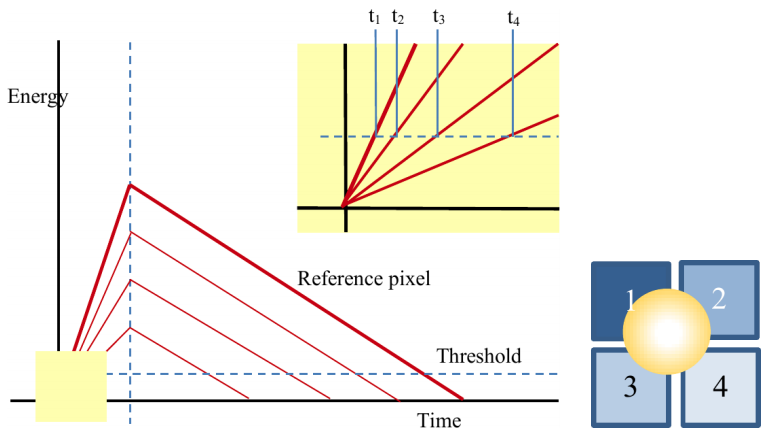
\includegraphics[width=12cm]{figures/calib_timeWalk.png}
		\caption{\textit{Time-walk} efekt: příklad interakce jedné částice se čtyřmi pixely detektoru, kde v každém pixelu byla deponována jiná energie, což na výstupů zesilovačů pixelů způsobilo jiné hodnoty napětí. Díky rozdílné charakteristice náběžné hrany pulzů byl treshold překročen v různých časech ($t_{1-4}$) \cite{Turecek2016TimeWakl}.}
		\label{fig:det:calib:timeWalk}
	\end{center}
\end{figure}

S použitím detektoru \textit{Timepix3}\cite{timepix3} je možné tuto energeticky závislou chybu eliminovat za použití kalibrační metody \cite{Turecek2016TimeWakl}, protože tento detektor umožňuje měřit v ToA a ToT módu současně. Tato kalibrační metoda spočívá v analytickém zpracování dat získaných z měření se zdrojem alfa částic (v \cite{Turecek2016TimeWakl} použito $^{241}$\texttt{Am}), které generuje clustery o velikosti maximálně čtyři pixely. Nejprve je však třeba potřeba energeticky zkalibrovat \ref{chap:detectors:calibration:energy}. 

O vybraných clusterech o velikosti 3 a 4 pixely pro $^{241}$\texttt{Am} víme, že součet jejich energií je $59.5keV$. Z clusteru je vybraný pixel s energií $30keV$, který je použit jako referenční (na \ref{chap:detectors:calibration:timeWalk} jako $t_1$), zbylá energie je náhodně rozdělena mezi ostatní pixely (na \ref{chap:detectors:calibration:timeWalk} jako $t_{2-4}$). Jednotlivé rozdíly $t_i+t_1$ jsou analytickými metodami, popsanými v \cite{Turecek2016TimeWakl}, zpracovány a výsledkem tohoto procesu jsou konstanty $c,d$ pro každý pixel detektoru, kterými lze vypočítat jeho \textit{Time-Walk offset} $\Delta T$:

\begin{equation}\label{eq:det:timeWalk}
	\Delta T = \frac{c}{(E - E_0)^d}
\end{equation}
kde:
\begin{changemargin}{1.5cm}{1cm} 
	\begin{itemize}
		\item [$\Delta T$] je \textit{Time-Walk} korekce pixelu [$ns$] (výsledná hodnota ToA je pak rovna $ToA-\Delta T$),
		\item [$E$] je energie pixelu [keV],
		\item [$E_0$] je treshold pixelu [keV] a
		\item [$c,d$] jsou konstanty.
	\end{itemize}
\end{changemargin}

\subsection{ToA offset korekce}\label{chap:detectors:calibration:toa_correction}
Jedná se o jev, ke kterému dochází u \textit{Timepix3} detektorů z důvodu chyby hardware, který způsobuje špatnou synchronizaci časového razítka napříč sloupci detektoru \cite{Katherine}. Tato chyba vzniká jen při zapnutí detektoru a poté je \texttt{ToA} offset již stabilní, takže je možné vytvořit korekci.

Odstranění tohoto jevu spočívá ve vytvoření kompenzační tabulku pomocí středních hodnot interních testovacích pulzů \cite{timepix3}. Pro získání správných hodnot \texttt{ToA} z naměřených dat stačí jen odečíst příslušnou hodnotu z korekční tabulky.

%********************************************************************************
% Přehled detektorů rodiny Medipix
%********************************************************************************
\section{Přehled detektorů rodiny Medipix}\label{chap:detectors:medipix_overview}
V této podkapitole budou stručně představeny jednotlivé detektory, které byly vyvinuty v rámci Medipix kolaborace \cite{medipix-www}.

\begin{description}

	\item[Medipix1] V roce 1998 byl vyvinut detektor \textit{Medipix1} \cite{medipix1}, také zvaný \textit{Photon-Counting-Chip}, byl první velkoplošný detektor používající CMOS technologie. S maticí $64\times64$ pixelů, každým o hraně $170~\mu m$, má celkovou aktivní plochu $1,1~cm^2$. I přes malý počet pixelů a jejich velkou rozteč, tento detektor prokázal dobré rozlišovací vlastnosti, především pak v rentgenovém zobrazování. 
	
	Detektor je vyrobený pomocí $1~\mu m$ technologie a je schopný operovat pouze v Medipix módu (viz \ref{fig:det:modes}) a podporuje pouze vyčítání po snímcích (viz \ref{chap:detectors:readout}).
	
	\item[Medipix2] V roce 2001 byl vyvinut detektor \textit{Medipix2} \cite{medipix2}, jako náhrada za svého předchůdce \textit{Medipix1}. Díky $250~nm$ technologii bylo možné zvýšit počet pixelů a zároveň snížit jejich rozteč - detektor má $256\times256$ pixelů, každý o hraně $55~\mu m$. Navíc má dva tresholdy s diskriminací na 4 pixely. 
	
	Stejně jako svůj předchůdce je schopný operovat pouze v Medipix módu (viz \ref{fig:det:modes}) a podporuje pouze vyčítání po snímcích (viz \ref{chap:detectors:readout}).
	
	\item[Timepix]\label{chap:detectors:medipix_overview:timepix} V roce 2006 byl vyvinut detektor \textit{Timepix} \cite{timepix}, který vychází z detektoru \textit{Medipix2}. Detektory mají stejné rozměry, ale architektura pixelů se změnila. Nově každý pixel detektoru umožňuje nezávisle měřit čas interakce částice, její energii, nebo je schopný počítat jednotlivé interakce. 
	
	Detektor je schopný operovat v \texttt{ToT}, \texttt{ToA}, nebo v Medipix módu (viz \ref{fig:det:modes}) a podporuje pouze vyčítání po snímcích (viz \ref{chap:detectors:readout}).
	
	\item[Medipix3] V roce 2011 byl vyvinut detektor \textit{Medipix3} \cite{medipix3}, jako nástupce \textit{Medipix2} detektoru. Rozměry detektoru zůstaly zachovány ($256\times256$ pixelů, každý o hraně $55~\mu m$), ale díky $130~nm$ technologii byla funkce jednotlivých pixelů vylepšena. Detektor nově umožňuje zvýšení energetického rozlišení díky potlačení \textit{Charge-Sharing} efektu (viz \ref{chap:detectors:calibration:energy}) pomocí integraci náboje do clusteru $4\times4$ pixelů. 
	
	Každý pixel má dva 14-bitové čítače. Jednotlivé pixely můžou být naprogramovány tak, aby vždy měřily za pomocí jednoho čítače, zatímco je hodnota z druhého čítače vyčítána, což umožňuje měření bez mrtvé doby.

	Také je možné zapojit tento readout čip (s pixelem o hraně $55~\mu m$) na senzor s pixely o hraně $110~\mu m$, takže výsledný super-pixel má k dispozici 8 čítačů a pomocí různých úrovní tresholdů jej lze použít jako 8-kanálový spektrometr.

	Stejně jako svůj předchůdce je schopný operovat pouze v Medipix módu (viz \ref{fig:det:modes}) a podporuje pouze vyčítání po snímcích (viz \ref{chap:detectors:readout}).

	\item[Timepix3]\label{chap:detectors:medipix_overview:timepix3} V roce 2014 byl vyvinut detektor \textit{Timepix3} \cite{timepix3}, jako nástupce \textit{Timepix} detektoru. Rozměry byly zachovány, ale bylo použita $130~\mu m$ výrobní technologie, jako u \textit{Medipix3}. Detektor nově umožňuje měřit v \texttt{ToA} a \texttt{ToT} současně a jeho časové rozlišení bylo vylepšeno více než na šestinásobek.

	Detektor nově umožňuje kromě vyčítání po snímcích i \textit{Data-Driven} mód, kde jsou data v rámci akvizice kontinuálně z detektoru vyčítána (viz \ref{chap:detectors:readout}). Takto navržená architektura umožňuje vyčítat data až do $40M_{hits}*cm^{-2}*s^{-1}$ bez globální mrtvé doby detektoru (pouze s lokální mrtvou dobou - pro jednotlivé pixely, ze kterých jsou vyčítána naměřená data).

	Na obrázku \ref{fig:det:medipix_overview:timepix3_schema} je znázorněno blokové schéma jednoho pixelu \textit{Timepix3} detektoru, který se skládá z analogové a digitální části (pro popis funkcionality viz \ref{chap:detectors:princip}). Na obrázku vpravo je pak společná elektronika, sdílená vždy 8 sousedními pixely (tzv.\textit{Super-pixel}).

\end{description}

\begin{figure}
	\begin{center}
		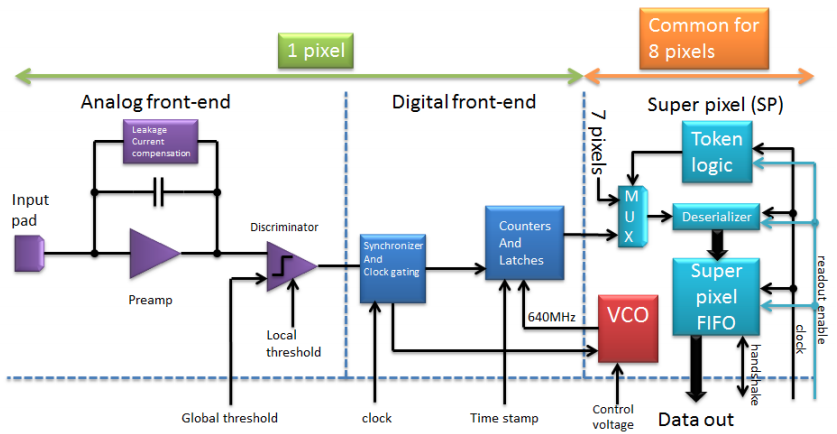
\includegraphics[width=15cm]{figures/det_timepix3_schema.png}
		\caption{Schéma pixelu detektoru \textit{Timepix3} se společnou elektronikou pro 8 pixelů (tzv.\textit{Super-pixel}) \cite{timepix3}.}
		\label{fig:det:medipix_overview:timepix3_schema}
	\end{center}
\end{figure}

%********************************************************************************
% Vyčítací rozhraní
%********************************************************************************
\section{Vyčítací rozhraní}\label{chap:detectors:readouts}
V této podkapitole bude popsáno několik vyčítacích rozhraní, které byly vyvinuty (v rámci \textit{Medipix kolaborace}\footnoteUrl{https://medipix.web.cern.ch}) ÚTEF ČVUT v Praze a jeho spinoff společností ADVACAM s.r.o. Pro komunikaci s \textit{Timepix3} detektorem bude v rámci této práce použito nově vyvinuté vyčítací rozhraní \textbf{Katherine} \cite{Katherine} \ref{chap:detectors:readouts:katherine}.

\subsection{FITPix}
FITPix \cite{fitpix} vyčítací rozhraní bylo vyvinuto v roce 2010 a skládá ze z programovatelného hradlového pole (\texttt{FPGA})\footnote{Z angl. Field Programmable Gate Array}, USB 2.0 rozhraní, DAC\footnote{Převodník digitálního signálu na analogový.} a ADC\footnote{Převodník analogového signálu na digitální.} převodníků a obvodů pro generování měřícího napětí (\textit{bias}).

Zařízení je s detektorem propojeno pomocí \textit{LVDS}\footnote{Z angl. Low-voltage differential signaling} a je schopné jeho plnohodnotného řízení, vč. nastavování hodnot (měřící frekvence, treshold, bias apod.), řízení akvizice a vyčítání naměřených dat rychlostí až $90$ snímků za sekundu. Zařízení rovněž umožňuje připojení externího trigger signálů pro synchronizované měření s více detektory současně.

FITPix je možné použít pouze jako nízkoúrovňové vyčítací rozhraní a veškerá business logika musí být implementována v připojeném počítači (např. deserializace a derandomizace naměřených dat apod.). Jako řídící software je použit \textit{Pixelman}\cite{pixelman}. Zařízení je kompatibilní se všemi detektory uvedenými v \ref{chap:detectors:medipix_overview}, kromě \textit{Timepix3}.

\subsection{AdvaDAQ}
AdvaDAQ \cite{Turecek2016TimeWakl} je nástupcem vyčítacího rozhraní FITPix a kompatibilní se všemi detektory uvedenými v \ref{chap:detectors:medipix_overview}. Principem funkce vychází ze svého předchůdce, ale díky použitému rozhraní USB 3.0 je schopné dosahovat maximálního datového toku $2,9~Gb/s$. Deserializace naměřených dat byla implementována do firmware \textit{FPGA}. Pro řízení tohoto rozhraní, vizualizaci a analýzu naměřených dat byl vyvinut software Pixet.

\subsection{ATLAS Pix}\label{chap:detectors:readouts:atlaspix}
ATLAS Pix \cite{atlastpx_sw, BegeraBcThesis2016} je zařízení vyvinuté v rámci experimentu \textit{ATLAS-TPX}, síti 16 hybridních částicových detektorů \textit{Timepix}, instalované v rámci experimentu \textit{ATLAS} na \textit{LHC} v \textit{CERN}, operující od roku 2014.

Zařízení vzniklo modifikací vyčítacího rozhraní \textit{FITPix} a disponuje \texttt{FPGA}, \texttt{LVDS} zesilovačem a počítače \textit{Raspberry Pi}, ve kterém je implementován software, poskytující API pro své vzdálené řízení přes \texttt{TPC} protokol. Komunikace mezi \texttt{FPGA} a počítačem je realizována pomocí \texttt{SPI}\footnote{Z angl. Serial Peripheral Interface.} protokolu.

\subsection{Katherine}\label{chap:detectors:readouts:katherine}
\begin{figure}
	\begin{center}
		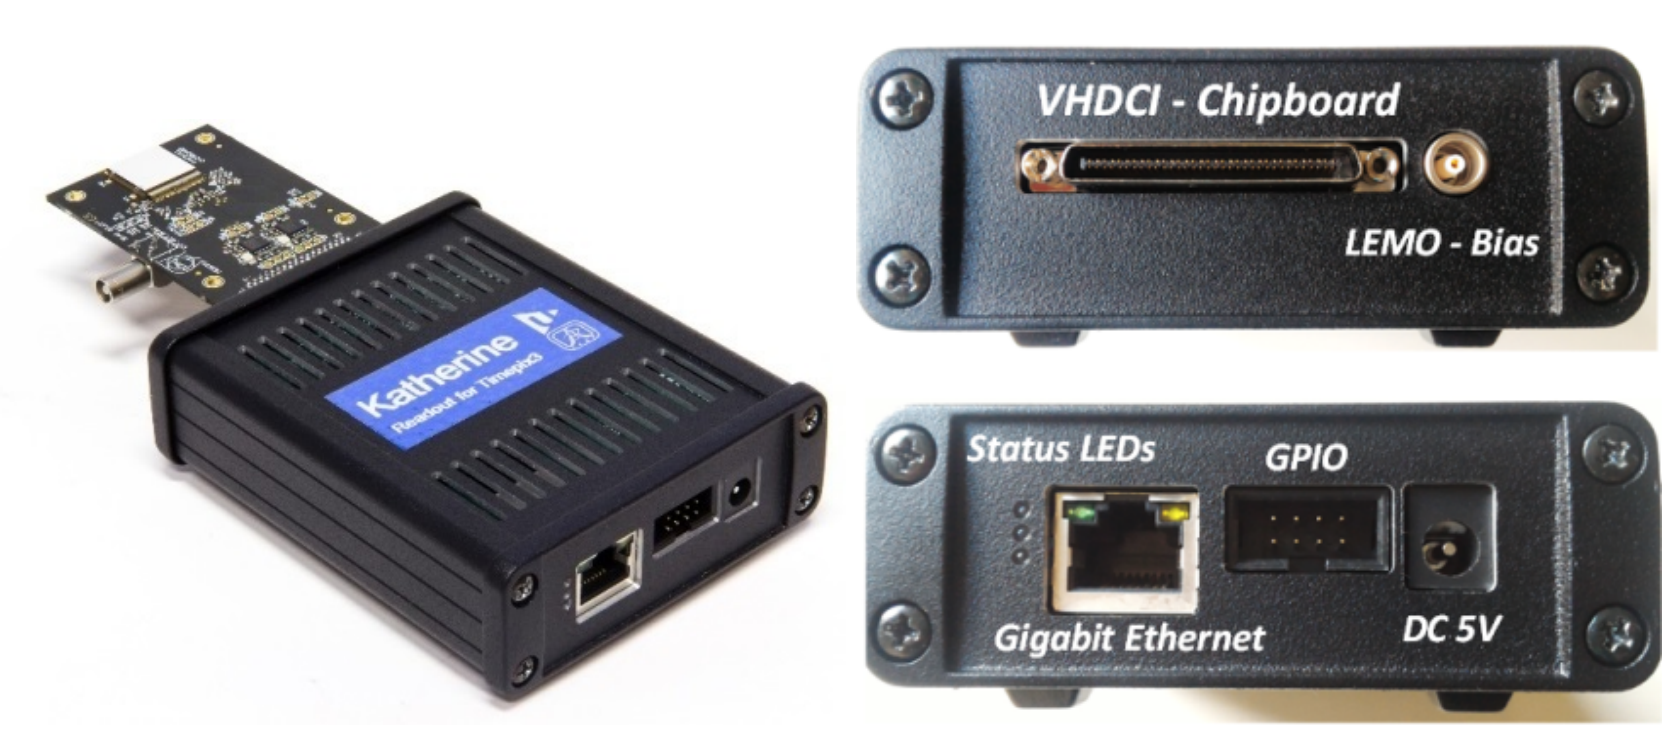
\includegraphics[width=15cm]{figures/det_katherine.png}
		\caption{Vyčítací rozhraní \textit{Katherine} s přípojeným detektorem \textit{Timepix3} vlevo a popisem vstupných a výstupních portů vpravo\cite{Katherine}.}
		\label{fig:det:readout:katherine}
	\end{center}
\end{figure}

Katherine \cite{Katherine} je pokročilé vyčítací rozhraní dedikované pro řízení jednoho \textit{Timepix3} detektoru, které v sobě obsahuje embedovaný počítač, čímž se vymezuje od ostatních vyčítacích rozhraní bez procesoru, kde business logika musí být implementována v připojeném počítači, což má negativní dopad na vytížení jeho procesoru. 

Hlavním benefitem zařízení je možnost jeho použití na experimentech, kde je nutná větší vzdálenost mezi detektorem a vyčítacím rozhraním (u \textit{Katherine až $100~m$}). Toto omezení je dáno především nedostatečnou radiační a elektromagnetickou odolností použité elektroniky. To umožňuje aplikace v blízkosti jaderných reaktorů nebo na částicových urychlovačích (například měření luminosity v rámci experimentu ATLAS na LHC v CERN \cite{atlastpx_luminosity}). 

Zařízení je kompatibilní s \textit{Timepix3} detektory, které jsou osazeny na CERN chipboard, nebo na kompatibilní \texttt{PCB}\footnote{Z angl. Printed Circuit Board.} s \texttt{VHDCI}\footnote{Z angl. Very-High-Density-Cable-Interconnect.} 68-pinovým konektorem. S detektorem může být propojeno napřímo (viz obr. \ref{fig:det:readout:katherine} vlevo), prodlužovacím \texttt{VHDCI} kabelem o maximální délce až $10~m$, nebo speciálním extenderem na bázi ethernetu pro vzdálenosti až $120~m$. S rostoucí vzdáleností ale klesá maximální datový tok (viz tabulka \ref{tab:det:katherine:data_flow}).

\begin{table}[th]
	\begin{center}
		\begin{tabular}{|c|c|c|c|}
			\hline
			\textbf{Vzdálenost} & \textbf{Typ propojení} & \textbf{Počet kanálů - datový tok} & \textbf{Hit Rate} \\
			\hline
			$3~m$ & VHDCI & $2 \times 640~Mb/s$ & $16~M_{hits}/s$\\
			$10~m$ & VHDCI & $4 \times 160~Mb/s$ & $10~M_{hits}/s$\\
			$20~m$ & Ethernet & $2 \times 640~Mb/s$ & $16~M_{hits}/s$\\
			$100~m$ & Ethernet & $4 \times 80~Mb/s$ & $5~M_{hits}/s$\\
			\hline
		\end{tabular}
	\end{center}
	\caption{Katherine: závislost maximálního datového toku na typu propojení mezi detektorem a vyčítacím rozhraním \cite{Katherine}.}
	\label{tab:det:katherine:data_flow}
\end{table}

Jeho maximální výstupní datový tok je daný použitým gigabitovým ethernetem, které odpovídá ekvivalentu datového toku $16M_{hits}*cm^{-2}*s^{-1}$ v \textit{Data-Driven} módu (viz \ref{chap:detectors:readout}). \textit{Timepix3} detektor je schopný generovat až $80M_{hits}*cm^{-2}*s^{-1}$, takže při vyšší zátěži není zařízení schopné přenést všechny zaznamenané události. Nicméně, \textit{Katherine} disponuje vestavěnou \texttt{DDR3} pamětí o velikosti $1~GB$, která funguje jako buffer - když je aktuální počet zpracovávaných událostí vyšší, než je maximální datový tok spojení s nadřazeným počítačem, tak se data hromadí v bufferu, aby později při nižší intenzitě zpracovávaných událostí mohly být přeneseny.

Pro úplnost výčtu vstupních a výstupných portů je třeba doplnit, že \textit{Katherine} také disponuje \texttt{GPIO}\footnote{Z angl. General Purpose Input/Output.} konektorem (viz obr. \ref{fig:det:readout:katherine} vpravo), zahrnující 4 obecné signály pro integraci s dalšími zařízeními a další rozšíření, jako například pro trigger synchronizaci (pro možnost zapojení například do detektorového teleskopu \cite{katherine_telescope}). Zařízení dále disponuje \texttt{LEMO} konektorem (viz \ref{fig:det:readout:katherine}), poskytujícím vysokonapěťový zdroj ($\pm300~V$) pro \textit{bias} (měřící napětí) detektoru.

Vyčítací rozhraní má implementovanou podporu pro \texttt{ToA} korekci (viz \ref{chap:detectors:calibration:toa_correction}), které je automaticky vykonána v rámci startovací sekvence, kde jsou poškozené sloupce identifikovány pomocí středních hodnot testovacích pulzů a je sestavena kompenzační tabulka. V průběhu akvizice dat jsou \texttt{ToA} hodnoty automaticky opraveny odečtením příslušných hodnot z výše zmíněné tabulky.

\subsubsection{Komunikace s nadřazeným PC a řízení akvizice dat}\label{chap:detectors:readouts:katherine:comm}
Vyčítací rozhraní \textit{Katherine} je dle dané konfigurace schopné operovat ve dvou módech:

\begin{description}
	\item [SFTP klient (autonomní mód)] V tomto módu zařízení operuje z pohledu řízení a akvizice dat zcela nezávisle. Po spuštění zařízení, resp. dokončení startovací sekvence, jsou z dodané konfigurace automaticky nastaveny měřící a akviziční parametry detektoru a je spuštěna akvizice dat. Získaná data jsou pak nepřetržitě posílána pomocí \textit{SFTP}\footnote{Z angl. Secure File Transfer Protocol (protokol pro zabezpečený přenos souborů mezi počítači pomocí \texttt{TPC} protokolu).} na server, kde jsou data ukládána do definovaného adresáře v \texttt{ASCII} souborech. Výhoda tohoto módu spočívá v jednoduchosti obsluhy a hodí se především pro takové aplikace, kde není očekáván vysoký datový tok a kde není potřeba měnit nastavení detektoru, protože každé jeho změna vyžaduje restart zařízení.
	
	\item [Manuální mód] Pracuje-li zařízení v tomto módu, pak k jeho funkci je třeba řízení z nadřazeného počítače pomocí proprietárního \texttt{UDP}\footnote{Z angl. User Datagram Protocol.} protokolu. Protokol využívá dvou \texttt{UDP} portů - \textbf{řídícího} a \textbf{datového}.

	\begin{description}
		\item [Komunikační] port je vyhrazen pro přenos řídících a konfiguračních paketů. Komunikace je implementována pomocí $36$ příkazů, kde každý z nich se skládá 64-bitového datagramu pro request a 64-bitového datagramu pro response, takže se jedná o synchronní potvrzovanou komunikaci\footnote{Potvrzování je realizováno na aplikační úrovni \texttt{ISO/OSI} modelu.}. Pro příklad viz obrázek \ref{tab:det:katherine:comm:packet_example}, kde je zobrazen request datagramu pro vyčtení biasu a jeho response.
		
		\item [Datový] port je určen pro jednosměrnou komunikaci z \textit{katherine} do nadřazeného počítače a slouží k přenosu naměřených dat. Každý datagram se skládá z 3-bitové hlavičky 43-bitových dat.
	\end{description}
	
\end{description}

\begin{figure}[]
	\begin{center}
		\begin{bytefield}[endianness=big,bitwidth=0.52em]{64}
			\begin{rightwordgroup}{Odchozí\\datagram}
				\bitheader{63,56,48,40,32,24,16,8,0} \\
				\bitbox{16}{\textbf{Command ID}} & \bitbox{48}{\textbf{Command data}} \\
				\bitbox{16}{0x0C} & \bitbox{8}{-} & \bitbox{8}{bias id} & \bitbox{32}{-}
			\end{rightwordgroup}
		\end{bytefield}
		
		\begin{bytefield}[endianness=big,bitwidth=0.52em]{64}
			\\ \\ \\
			\begin{rightwordgroup}{Příchozí\\datagram}
				\bitheader{63,56,48,40,32,24,16,8,0} \\
				\bitbox{16}{\textbf{Command ID}} & \bitbox{48}{\textbf{Command data}} \\
				\bitbox{16}{0x0C} & \bitbox{16}{-} & \bitbox{32}{bias (float)}
			\end{rightwordgroup}
		\end{bytefield}
	\end{center}
	\caption{Katherine: příklad requestu a response řídícího datagramu pro vyčtení biasu.}
	\label{tab:det:katherine:comm:packet_example}
\end{figure}

V rámci této práce bude použit druhý zmíněný - manuální mód, protože je méně náročný na šířku pásma a umožňuje vzdálené řízení detektoru. V dalších kapitolách (viz \todo ref) bude komunikační rozhraní vyčítacího rozhraní \textit{Katherine} popsáno podrobněji.